\section{Introduction}\label{chap:intro}

Within the financial industry, identifying and mitigating risks emerge as paramount concerns. The inherent uncertainty in the market engenders multifaceted manifestations of risk. Notably, liquidity, market, and credit risks are particularly consequential (\cite{hull2012risk}). Each risk category considers discrete origins of uncertainty, thereby necessitating the formulation of corresponding models. This study focuses on the sphere of market risk concerning the option market.

Market risk\footnote{Throughout this study, we employ Value-at-Risk (VaR) as the primary risk measure for market risk assessment. However, it is essential to note that the methods presented in this research allow for the estimation of the empirical distribution of portfolio value changes, enabling the calculation of both VaR and Expected Shortfall (ES).}, stemming from the uncertainty of market price fluctuations, is a widely acknowledged concern in equities and fixed-income securities. However, regarding derivatives, risk assessment becomes notably more complex. This study is dedicated to risk analysis, specifically emphasizing European options associated with non-dividend-paying stocks. Two primary approaches are utilized to estimate market risk effectively in the context of options: Historical Simulation (HS) and Parametric Estimation.

Historical simulation is a straightforward method for estimating VaR in option portfolios, using real market data to capture non-normal return distributions. It facilitates scenario analysis (\cite{hull2012risk}) to understand portfolio performance under various market conditions. However, its accuracy depends on data quality and doesn't consider forward-looking information or market dynamics changes. It assumes past statistical properties persist into the future, and it may be challenging to apply to illiquid assets or limited trading history (\cite{pritsker2006hidden}). Additionally, it's constrained by historical data length. Combining it with other VaR methods can mitigate these limitations, which we have also done.

The parametric approach in risk estimation focuses primarily on the underlying pricing model and endeavors to predict and estimate VaR by leveraging structural information. Initially, this approach entails calibrating the chosen model, providing valuable insights into the model's parameters. Subsequently, following the calibration procedure, the calculation of VaR is executed through conditional simulation (\cite{glasserman2000efficient}). As such, the parametric approach often employs the Monte Carlo (MC) method in conjunction with it. The estimation of VaR is rooted in the empirical distribution of returns, which is adjusted or conditioned based on the outcomes derived from the calibration process. This conditioning step aims to account for potential alterations in market dynamics, volatility levels, or correlations, which might not be adequately captured through the simplistic historical simulation approach.

The Black-Scholes model within the framework of parametric estimation is the cornerstone of our research. The introduction of the pricing model by \cite{black1973pricing} marked a seminal advancement in trading European option contracts. This specific model relies on several simplifying assumptions akin to various models. Notably, the constant volatility in the underlying asset constitutes one such assumption, a facet that scholars endeavored to incorporate into the broader Black-Scholes framework in subsequent years. 

In the context of portfolio analysis, the absence of uncertainty related to volatility prompted the development of VaR models. Examples of such models include the Delta-Gamma method introduced by \cite{jorion2007value} and the straightforward one-day Monte Carlo method. In both approaches, volatility is considered constant over a single period, resulting in negligible volatility-driven risk within that timeframe. However, these calculations may lack precision due to the simplifying assumption of constant volatility inherent in the Black-Scholes model. 

Historical data frequently reveals that asset price volatility is not consistent but rather fluctuates between high and low volatility periods. \cite{mandelbrot1967distribution} initially introduced this concept in their pioneering research. Hence, while the Black-Scholes model provides reasonable estimates for many options, it may produce inaccurate results when applied to options on assets with highly variable or stochastic volatility, such as during financial crises or significant news events. Additionally, historical events, including the notorious Black Monday of 1987, prompted market participants to reevaluate their reliance on this model (\cite{hull2003options}). These events engendered a realization that the model might need to be more aptly suited to account for the considerable fluctuations and volatility witnessed in the underlying asset. Consequently, the applicability of the Black-Scholes model comes into question in situations marked by significant market turbulence, potentially leading traders utilizing this framework to face considerable financial losses. 
\begin{figure}
    \centerline{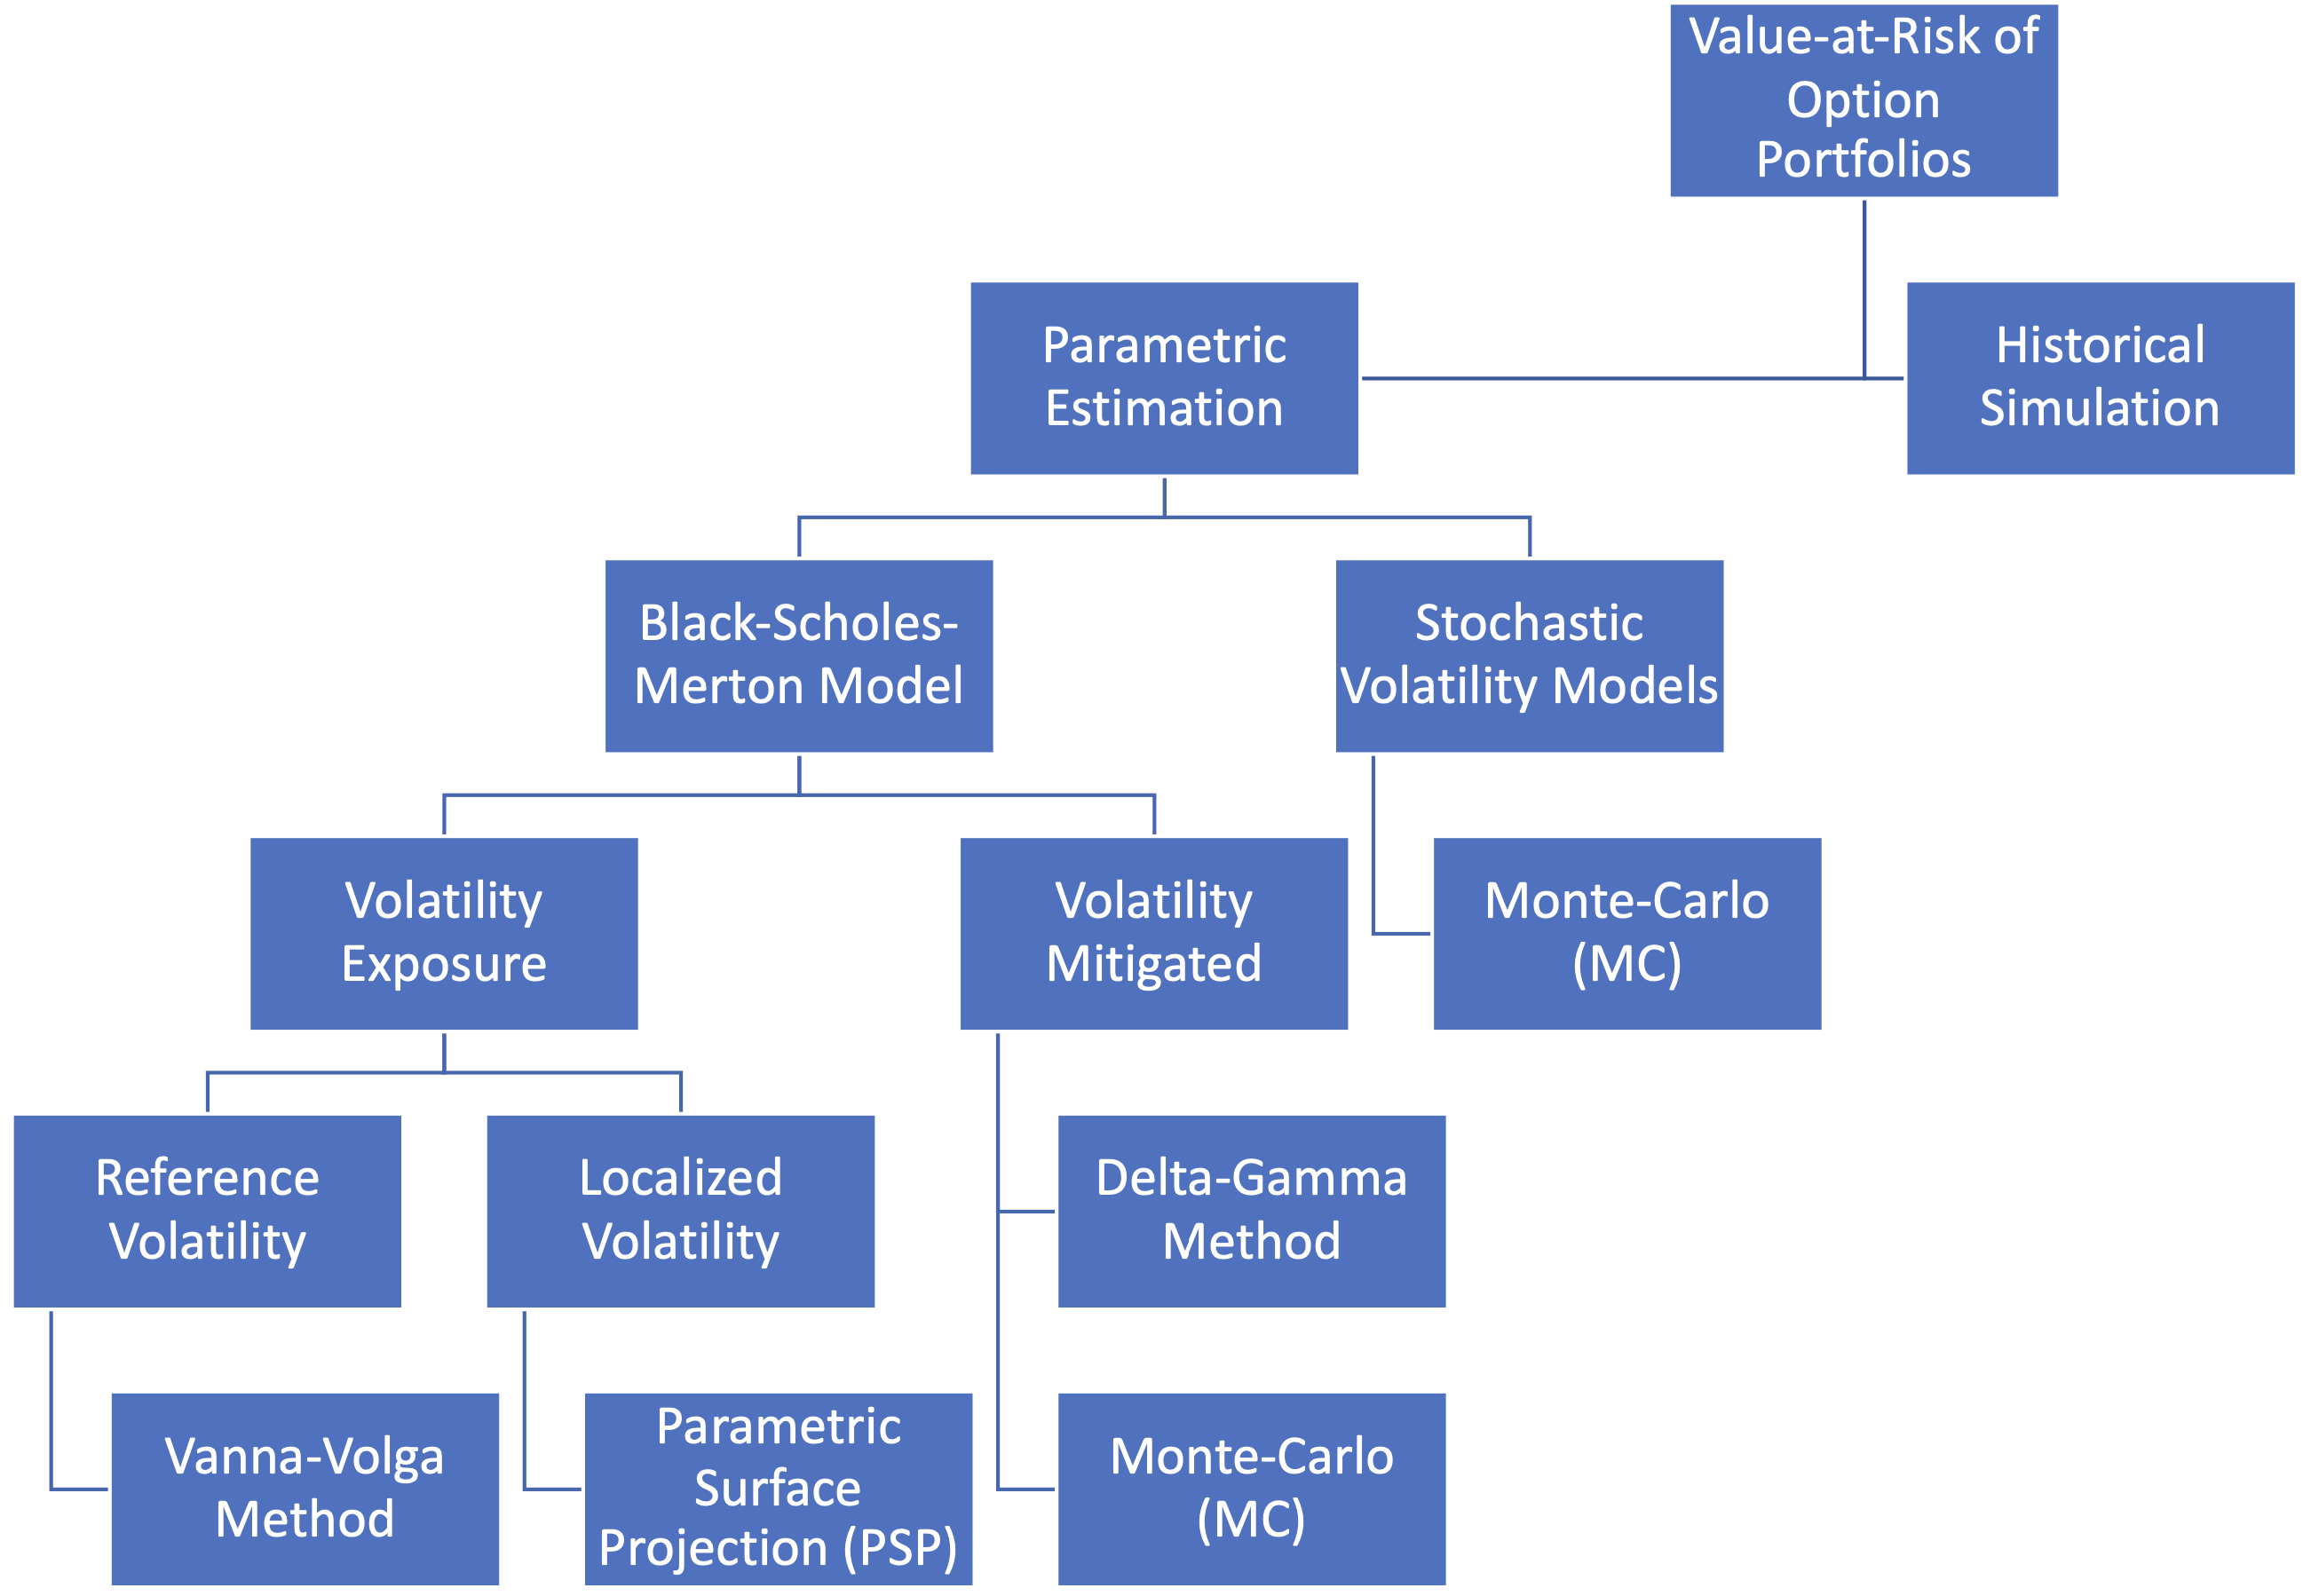
\includegraphics[width=\linewidth]{figs/Intro_Models.png}}
    \caption{This figure illustrates the proposed hierarchy of VaR calculation methods within option portfolios, as introduced in the introduction. It is important to note that the hierarchy does not imply any temporal precedence of one method over another. Instead, it visually represents how our suggested model relates to other methods in this context.}
    \label{fig:Intro_Models}
\end{figure}

In response to the limitations associated with the constant volatility assumption, options pricing has developed advanced models to refine methodologies. Notable contributions in this regard include \cite{hull1987pricing} and \cite{dupire1997pricing} pioneering researches, introducing stochastic volatility and local volatility models, respectively. These models represent significant strides toward reconciling the disparities arising from constant volatility assumptions when juxtaposed with the intricate dynamics of real-world markets.

However, the introduction of such advanced models has brought forth new challenges. Calibration processes for these models can be highly intricate, demanding a nuanced approach. Additionally, accurately forecasting the temporal fluctuations in volatility remains a formidable task, as highlighted in \cite{Verma2008ImpliedVM}. Furthermore, there are concerns regarding the compatibility of these advanced models with the second fundamental law of asset pricing, as discussed by \cite{clark2011foreign}.

Despite these challenges, these models offer promising avenues for addressing the volatility-related uncertainties intrinsic to options pricing. Moreover, in estimating VaR, these models often involve conditional simulation methods within the Monte Carlo framework, enhancing their applicability in capturing the dynamic nature of financial markets.

Researchers and market participants often employ implied volatility within the Black-Scholes framework to harness the simplicity of the Black-Scholes model and address the uncertainties stemming from volatility changes. Implied volatility serves as a means to gauge anticipated future volatility in the underlying asset, thus constituting a pivotal component of the Black-Scholes model. This estimation draws from the market prices of options, prompting market participants to base option quotations on their implied volatility rather than relying solely on prevailing market pricing (\cite{hull2003options}).

\cite{carr2020option} influential work delineates two distinct approaches for assessing option risks within the Black-Scholes framework: the reference volatility model and localized volatility models. 

The reference volatility model is designed to establish a consistent pricing framework applicable to a broad spectrum of options by introducing the concept of reference volatility. For example, in their study, \cite{mercuriovanna} employed the vanna-volga model to delve into Black-Scholes pricing, subsequently facilitating VaR calculations. This model incorporates the idea of reference volatility, offering a systematic approach to pricing various options.

On the contrary, localized volatility models pivot on the implied volatility of individual options, aiming to deduce pricing implications without a deep understanding of the underlying rationale. Within this context, \cite{carr2020option} introduced the top-down valuation approach, while \cite{arslan2009gamma} and \cite{gershon2018model} extended the vanna-volga framework. These methodologies collectively integrate the implied volatility of individual options into the valuation process. This enables a more nuanced assessment of option pricing dynamics, providing insights into market sentiment and potential mispricings.

Consistent with the premise outlined by \cite{carr2020option}, this study aims to deepen our understanding of the impact of volatility fluctuations on option portfolios. We have employed the localized volatility model framework to achieve this objective, utilizing the Implied Volatility Surface (IVS). This concept could prove highly advantageous for regulators due to its straightforward implementation while maintaining sufficient accuracy to prevent substantial financial losses.

Implied volatility, a cornerstone of the Black-Scholes pricing model, demonstrates variations across diverse levels of moneyness\footnote{The concept of moneyness in the context of options refers to the current state of an option relative to the prevailing market conditions, with a specific focus on the option's strike price (K) and the present market price of the underlying asset (S). In this study, moneyness for call options is calculated as the ratio $\frac{S}{K}$.} and time-to-maturity, culminating in forming a three-dimensional construct termed the implied volatility surface (IVS), as shown in Figure \ref{fig:IVS(2013_01_10)}. This dynamic surface, analogous to the yield curve (\cite{zamani2022pathwise}), encounters temporal fluctuations (Figure \ref{fig:IVStwo_dates}). Similarities to the yield curve are discernible in the IVS variations, albeit accompanied by the additional complexities introduced by an extra dimension and the variable nature of sample points within the IVS (\cite{skiadopoulos2000dynamics}). Functional representation has emerged as an alternative to point-based methodologies to circumvent challenges tied to sample point adjustments on the IVS. Further intricacies inherent to this phenomenon will be expounded upon in subsequent sections.
\begin{figure}
    \centerline{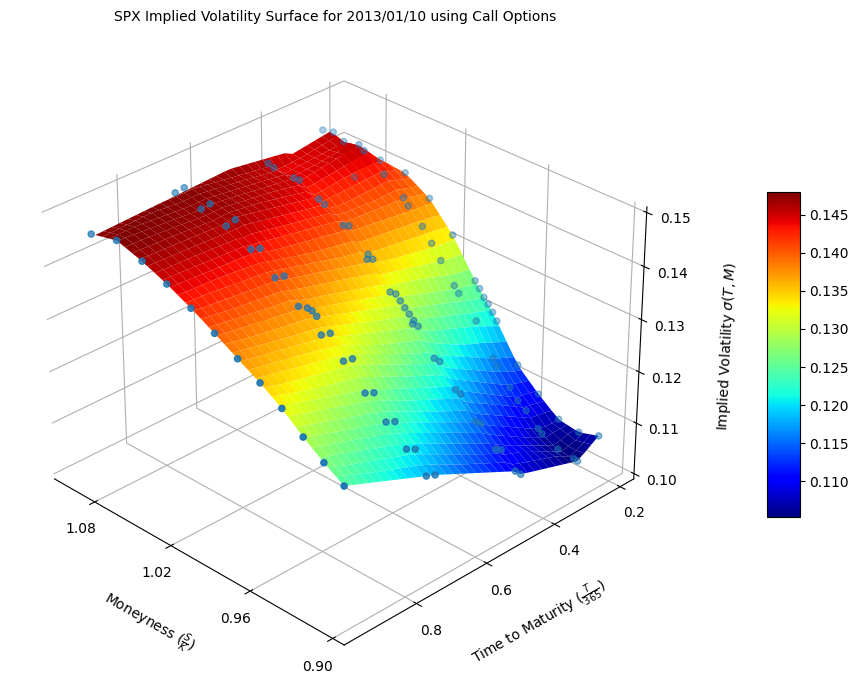
\includegraphics[width=0.9\linewidth]{figs/IVSlinear2013_01_10.png}}
    \caption{On January 10, 2013, an examination of implied volatility was conducted across various call options, considering different expiration dates and strike prices. This analysis effectively rejected the hypothesis of constant volatility. The graphical representation of this analysis featured two axes: one is moneyness denoted as $\frac{S}{K}$, where $K$ represents the strike price, and $S$ signifies the underlying asset price. The other is the time-to-maturity of the options, measured in years. Furthermore, the data points available on the volatility surface correspond to the observed implied volatility for the various options under examination.}
    \label{fig:IVS(2013_01_10)}
\end{figure}
\begin{figure}
    \centerline{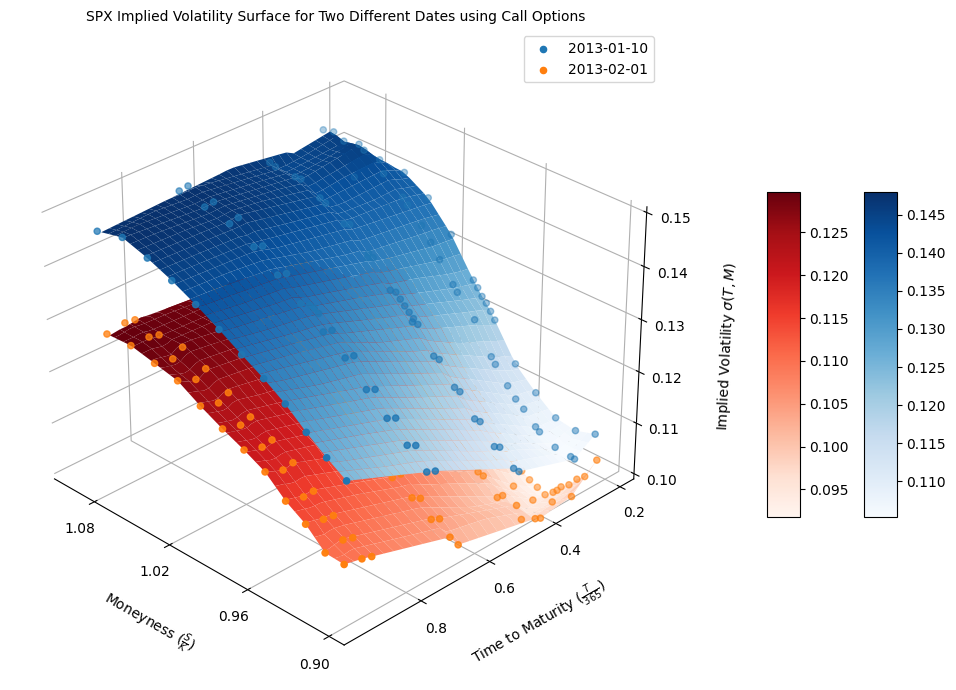
\includegraphics[width=\linewidth]{figs/IVSlineartwo_dates.png}}
    \caption{This Figure presents the Implied Volatility Surface (IVS) of the S\&P 500 index for two distinct dates. The Implied Volatility Surface (IVS) exhibits dynamic characteristics, shifting and altering its shape as the time parameter changes. This dynamism results in a lack of a fixed form for the Implied Volatility Surface (IVS) at any specific moment. Instead, it highlights the inherently uncertain nature of the Implied Volatility Surface (IVS). Again, the data points available on the volatility surface correspond to the observed implied volatility for the various options under examination.}
    \label{fig:IVStwo_dates}
\end{figure}

We introduce an innovative parametric surface projection methodology, harnessing historical simulation and Monte Carlo techniques. We construct a Profit and Loss (P\&L) distribution by scrutinizing historical observations, enabling the VaR computation. The effectiveness of the proposed approach is subsequently evaluated utilizing data extracted from the U.S. option database\footnote{The data used in this study was sourced from the U.S. option database, accessible at \url{https://optiondata.org/\#sampleId}. It is important to note that only the free data from the website was utilized in the analysis.}. To fulfill this objective, we draw upon established models from the contemporary academic corpus, which have been developed to appraise the methodologies employed for VaR calculations (\cite{roccioletti2015backtesting}).

The dynamic changes observed within the IVS are pivotal factors that significantly impact the pricing dynamics of options contracts. These alterations in IVS are consequential in risk assessment and management within financial markets. These deviations are not unique to a single market but are also evident in the currency market. 

For instance, we can observe similar phenomena in the realm of foreign exchange (FX). The FX implied forward curve is a valuable indicator that reflects market expectations concerning future borrowing rates. Employing parametric projection techniques based on historical scenarios becomes particularly relevant to understand better and leverage these expectations for risk assessment and decision-making.

In summary, the suggested method is not limited to a specific financial domain but extends its influence across various markets, including the currency market. Utilizing parametric projections based on historical scenarios can be a valuable approach to harnessing these dynamics for risk assessment and pricing in these markets.

The subsequent sections of this work are outlined below. Section \ref{sec:Methodology} presents our methodology for estimating the Value at Risk (VaR) arising from IVS movements of option portfolios. In Section \ref{results}, an evaluation of our strategy is conducted utilizing a range of tests and models. The section \ref{conclusion} of the study is brought to a close.